\documentclass[aspectratio=169]{beamer}

% === Theme Configuration ===
\usetheme{Madrid}
\usecolortheme{whale}
\setbeamertemplate{navigation symbols}{}
\setbeamertemplate{footline}[frame number]

% === Packages ===
\usepackage[utf8]{inputenc}
\usepackage[romanian]{babel}
\usepackage{amsmath,amsfonts,amssymb}
\usepackage{graphicx}
\usepackage{listings}
\usepackage{xcolor}
\usepackage{tikz}
\usetikzlibrary{shapes,arrows,positioning,calc}
\usepackage{hyperref}
\usepackage{booktabs}
\usepackage{multicol}

% === Colors ===
\definecolor{codegreen}{rgb}{0,0.6,0}
\definecolor{codegray}{rgb}{0.5,0.5,0.5}
\definecolor{codepurple}{rgb}{0.58,0,0.82}
\definecolor{backcolour}{rgb}{0.95,0.95,0.92}

% === Code Listings ===
\lstdefinestyle{codestyle}{
    backgroundcolor=\color{backcolour},
    commentstyle=\color{codegreen},
    keywordstyle=\color{magenta},
    numberstyle=\tiny\color{codegray},
    stringstyle=\color{codepurple},
    basicstyle=\ttfamily\scriptsize,
    breakatwhitespace=false,
    breaklines=true,
    captionpos=b,
    keepspaces=true,
    numbers=left,
    numbersep=5pt,
    showspaces=false,
    showstringspaces=false,
    showtabs=false,
    tabsize=2
}
\lstset{style=codestyle}

% === Title Information ===
\title[Simulare OTP]{Simularea unui Mecanism One-Time Pad}
\subtitle{Proiect Criptografie}
\author{Student}
\institute{Facultatea de Informatică}
\date{\today}

\begin{document}

% === Title Slide ===
\begin{frame}
    \titlepage
\end{frame}

% === Outline ===
\begin{frame}{Cuprins}
    \tableofcontents
\end{frame}

% ============================================================
\section{Introducere în Criptografie}
% ============================================================

\begin{frame}{Ce este Criptografia?}
    \begin{columns}
        \begin{column}{0.5\textwidth}
            \textbf{Definiție:}
            \begin{itemize}
                \item Știința comunicării secrete
                \item Transformarea informației pentru protecție
                \item Asigurarea confidențialității
            \end{itemize}

            \vspace{0.5cm}
            \textbf{Terminologie:}
            \begin{itemize}
                \item \textbf{Plaintext} (M) - mesaj original
                \item \textbf{Ciphertext} (C) - mesaj criptat
                \item \textbf{Key} (K) - cheie secretă
                \item \textbf{Encryption}: $E_K(M) = C$
                \item \textbf{Decryption}: $D_K(C) = M$
            \end{itemize}
        \end{column}
        \begin{column}{0.5\textwidth}
            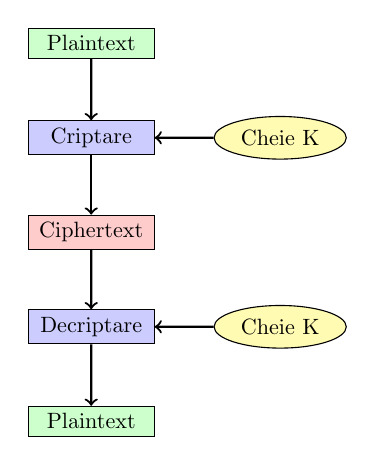
\begin{tikzpicture}[node distance=1.5cm, auto, scale=0.8, transform shape]
                \node[draw, rectangle, fill=green!20, minimum width=2cm] (plain) {Plaintext};
                \node[draw, rectangle, fill=blue!20, minimum width=2cm, below of=plain] (enc) {Criptare};
                \node[draw, rectangle, fill=red!20, minimum width=2cm, below of=enc] (cipher) {Ciphertext};
                \node[draw, rectangle, fill=blue!20, minimum width=2cm, below of=cipher] (dec) {Decriptare};
                \node[draw, rectangle, fill=green!20, minimum width=2cm, below of=dec] (plain2) {Plaintext};
                \node[draw, ellipse, fill=yellow!30, right of=enc, xshift=1.5cm] (key1) {Cheie K};
                \node[draw, ellipse, fill=yellow!30, right of=dec, xshift=1.5cm] (key2) {Cheie K};

                \draw[->, thick] (plain) -- (enc);
                \draw[->, thick] (enc) -- (cipher);
                \draw[->, thick] (cipher) -- (dec);
                \draw[->, thick] (dec) -- (plain2);
                \draw[->, thick] (key1) -- (enc);
                \draw[->, thick] (key2) -- (dec);
            \end{tikzpicture}
        \end{column}
    \end{columns}
\end{frame}

\begin{frame}{Criptarea Simetrică}
    \begin{block}{Definiție}
        Utilizează \textbf{aceeași cheie} atât pentru criptare cât și pentru decriptare.
    \end{block}

    \vspace{0.5cm}
    \begin{columns}
        \begin{column}{0.5\textwidth}
            \textbf{Avantaje:}
            \begin{itemize}
                \item Rapidă și eficientă
                \item Algoritm simplu
                \item Nu necesită putere de calcul mare
            \end{itemize}
        \end{column}
        \begin{column}{0.5\textwidth}
            \textbf{Dezavantaje:}
            \begin{itemize}
                \item Problema distribuției cheilor
                \item Cheia trebuie partajată în siguranță
                \item Fiecare pereche de utilizatori necesită o cheie unică
            \end{itemize}
        \end{column}
    \end{columns}

    \vspace{0.5cm}
    \begin{center}
        \textbf{One-Time Pad este un sistem de criptare simetrică}
    \end{center}
\end{frame}

% ============================================================
\section{One-Time Pad (OTP)}
% ============================================================

\begin{frame}{One-Time Pad - Prezentare}
    \begin{block}{Definiție}
        One-Time Pad este singurul sistem de criptare cu \textbf{securitate perfectă} demonstrată matematic (Shannon, 1949).
    \end{block}

    \vspace{0.3cm}
    \textbf{Istoric:}
    \begin{itemize}
        \item Inventat de Gilbert Vernam în 1917
        \item Demonstrat de Claude Shannon în 1949
        \item Folosit în comunicații diplomatice și militare
    \end{itemize}

    \vspace{0.3cm}
    \textbf{Principiul de funcționare:}
    \begin{itemize}
        \item Fiecare byte din mesaj este combinat cu byte-ul corespunzător din cheie
        \item Operația folosită: \textbf{XOR} (sau exclusiv)
        \item Cheia trebuie să fie aleatorie și de lungimea mesajului
    \end{itemize}
\end{frame}

\begin{frame}{Formula Matematică OTP}
    \begin{alertblock}{Criptare și Decriptare}
        \begin{center}
            $C_i = M_i \oplus K_i$ \quad (Criptare)

            \vspace{0.3cm}
            $M_i = C_i \oplus K_i$ \quad (Decriptare)
        \end{center}
        unde $\oplus$ reprezintă operația XOR
    \end{alertblock}

    \vspace{0.5cm}
    \textbf{Notații:}
    \begin{itemize}
        \item $M_i$ = byte-ul $i$ din mesajul original
        \item $K_i$ = byte-ul $i$ din cheie
        \item $C_i$ = byte-ul $i$ din mesajul criptat
    \end{itemize}

    \vspace{0.3cm}
    \begin{exampleblock}{Observație importantă}
        Aceeași operație (XOR cu cheia) funcționează atât pentru criptare cât și pentru decriptare!
    \end{exampleblock}
\end{frame}

% ============================================================
\section{Operația XOR}
% ============================================================

\begin{frame}{Operația XOR - Fundament OTP}
    \begin{columns}
        \begin{column}{0.5\textwidth}
            \textbf{Tabel de adevăr XOR:}
            \begin{center}
                \begin{tabular}{|c|c|c|}
                    \hline
                    \textbf{A} & \textbf{B} & \textbf{A $\oplus$ B} \\
                    \hline
                    0 & 0 & 0 \\
                    0 & 1 & 1 \\
                    1 & 0 & 1 \\
                    1 & 1 & 0 \\
                    \hline
                \end{tabular}
            \end{center}

            \vspace{0.5cm}
            \textbf{Proprietăți importante:}
            \begin{itemize}
                \item $A \oplus A = 0$ (auto-inversă)
                \item $A \oplus 0 = A$ (element neutru)
                \item $(A \oplus B) \oplus B = A$ (reversibilă)
            \end{itemize}
        \end{column}
        \begin{column}{0.5\textwidth}
            \textbf{Exemplu practic:}
            \begin{align*}
                M &= \text{01001000} \quad (\text{'H'}) \\
                K &= \text{10101010} \quad (\text{cheie}) \\
                \hline
                C &= \text{11101010} \quad (\text{criptat})
            \end{align*}

            \textbf{Decriptare:}
            \begin{align*}
                C &= \text{11101010} \\
                K &= \text{10101010} \\
                \hline
                M &= \text{01001000} \quad (\text{'H'})
            \end{align*}
        \end{column}
    \end{columns}
\end{frame}

\begin{frame}{De ce funcționează XOR pentru criptare?}
    \begin{block}{Proprietatea cheie: Reversibilitate}
        $(A \oplus B) \oplus B = A$
    \end{block}

    \vspace{0.5cm}
    \textbf{Demonstrație:}
    \begin{enumerate}
        \item Criptare: $C = M \oplus K$
        \item Decriptare: $C \oplus K = (M \oplus K) \oplus K = M \oplus (K \oplus K) = M \oplus 0 = M$
    \end{enumerate}

    \vspace{0.5cm}
    \textbf{Avantaje XOR:}
    \begin{itemize}
        \item Operație foarte rapidă (la nivel de CPU)
        \item Reversibilă fără informații suplimentare
        \item Fiecare bit de output depinde de bit-ul de input și cheie
    \end{itemize}
\end{frame}

% ============================================================
\section{Securitate Perfectă}
% ============================================================

\begin{frame}{Condiții pentru Securitate Perfectă}
    \begin{block}{Teorema lui Shannon (1949)}
        Un sistem criptografic are securitate perfectă dacă și numai dacă:
        \begin{enumerate}
            \item Cheia este complet \textbf{aleatorie}
            \item Cheia are cel puțin \textbf{lungimea mesajului}
            \item Cheia nu este \textbf{refolosită niciodată}
            \item Cheia este păstrată \textbf{secretă}
        \end{enumerate}
    \end{block}

    \vspace{0.5cm}
    \begin{columns}
        \begin{column}{0.5\textwidth}
            \textbf{De ce securitate perfectă?}
            \begin{itemize}
                \item Ciphertextul nu dezvăluie informații
                \item Toate mesajele sunt la fel de probabile
                \item Imposibil de spart cu orice putere de calcul
            \end{itemize}
        \end{column}
        \begin{column}{0.5\textwidth}
            \textbf{Dezavantaje practice:}
            \begin{itemize}
                \item Distribuția securizată a cheilor
                \item Stocarea cheilor mari
                \item O singură utilizare per cheie
            \end{itemize}
        \end{column}
    \end{columns}
\end{frame}

\begin{frame}{Pericolul Reutilizării Cheii}
    \begin{alertblock}{ATENȚIE: Key Reuse Attack}
        Dacă aceeași cheie K este folosită pentru două mesaje diferite:
        \begin{align*}
            C_1 &= M_1 \oplus K \\
            C_2 &= M_2 \oplus K \\
            C_1 \oplus C_2 &= M_1 \oplus M_2
        \end{align*}
    \end{alertblock}

    \vspace{0.3cm}
    \textbf{Consecințe:}
    \begin{itemize}
        \item XOR-ul celor două ciphertexturi elimină cheia
        \item Atacatorul obține XOR-ul plaintexturilor
        \item Poate recupera mesajele prin analiza de frecvență
    \end{itemize}

    \vspace{0.3cm}
    \begin{exampleblock}{Exemplu istoric}
        \textbf{Proiectul VENONA} - NSA a spart mesaje sovietice datorită reutilizării cheilor OTP în anii 1940.
    \end{exampleblock}
\end{frame}

% ============================================================
\section{Implementarea Aplicației}
% ============================================================

\begin{frame}{Arhitectura Aplicației}
    \begin{center}
        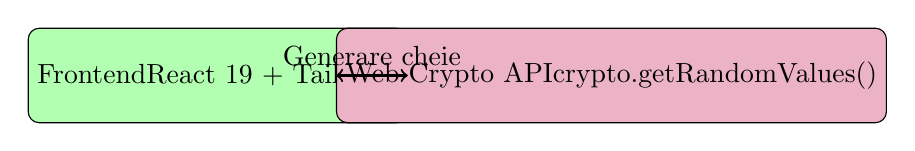
\begin{tikzpicture}[
            node distance=2cm,
            box/.style={draw, rectangle, rounded corners, minimum width=3.5cm, minimum height=1.2cm, fill=blue!20}
        ]
            \node[box, fill=green!30] (frontend) {Frontend\\React 19 + Tailwind};
            \node[box, fill=purple!30, right of=frontend, xshift=3cm] (crypto) {Web Crypto API\\crypto.getRandomValues()};

            \draw[->, thick, <->] (frontend) -- node[above] {Generare cheie} (crypto);
        \end{tikzpicture}
    \end{center}

    \vspace{0.5cm}
    \textbf{Tehnologii folosite:}
    \begin{itemize}
        \item \textbf{React 19} - framework JavaScript modern
        \item \textbf{Tailwind CSS} - framework CSS pentru stilizare
        \item \textbf{crypto.getRandomValues()} - generare numere aleatoare criptografic securizate
        \item \textbf{Hooks} - useState, useCallback pentru state management
    \end{itemize}
\end{frame}

\begin{frame}[fragile]{Implementare OTP în JavaScript}
\begin{lstlisting}[language=JavaScript, caption=Funcții principale OTP]
// generare cheie aleatorie securizata
const generateKey = (length) => {
  const key = new Uint8Array(length)
  crypto.getRandomValues(key)
  return key
}

// operatia xor pentru criptare/decriptare
const xorEncrypt = (messageBytes, keyBytes) => {
  const result = new Uint8Array(messageBytes.length)
  for (let i = 0; i < messageBytes.length; i++) {
    result[i] = messageBytes[i] ^ keyBytes[i]
  }
  return result
}
\end{lstlisting}

\textbf{Notă:} \texttt{crypto.getRandomValues()} este echivalent cu \texttt{crypto/rand} din Go.
\end{frame}

\begin{frame}{Funcționalități Implementate}
    \textbf{Aplicația oferă:}

    \begin{enumerate}
        \item \textbf{Input mesaj} - utilizatorul introduce un text
        \item \textbf{Generare cheie} - cheie aleatorie de lungimea mesajului
        \item \textbf{Criptare XOR} - aplicarea operației XOR
        \item \textbf{Afișare rezultate}:
            \begin{itemize}
                \item Mesaj original: text, ASCII, hexazecimal
                \item Cheie OTP: hexazecimal
                \item Mesaj criptat: hexazecimal
                \item Mesaj decriptat: text, ASCII, hexazecimal
            \end{itemize}
        \item \textbf{Verificare} - confirmă că decriptarea = originalul
        \item \textbf{Salvare fișiere} - export cheie și mesaj criptat
    \end{enumerate}
\end{frame}

\begin{frame}{Formate de Afișare}
    \begin{table}
        \centering
        \begin{tabular}{|l|l|l|}
            \hline
            \textbf{Format} & \textbf{Descriere} & \textbf{Exemplu ("ABC")} \\
            \hline
            Text & Caracterele originale & ABC \\
            \hline
            ASCII & Coduri ASCII (decimal) & 65 66 67 \\
            \hline
            Hexazecimal & Valori hex & 41 42 43 \\
            \hline
        \end{tabular}
    \end{table}

    \vspace{0.5cm}
    \textbf{De ce multiple formate?}
    \begin{itemize}
        \item \textbf{Text} - pentru înțelegere umană
        \item \textbf{ASCII} - pentru a vedea valorile numerice
        \item \textbf{Hex} - standard în criptografie, compact
    \end{itemize}
\end{frame}

% ============================================================
\section{Demonstrație}
% ============================================================

\begin{frame}{Exemplu de Utilizare}
    \textbf{Pas 1: Introducem mesajul "SALUT"}

    \vspace{0.3cm}
    \textbf{Pas 2: Se generează cheie aleatorie}

    \vspace{0.3cm}
    \textbf{Pas 3: Rezultate afișate:}

    \begin{table}
        \centering
        \begin{tabular}{|l|l|}
            \hline
            \textbf{Câmp} & \textbf{Valoare} \\
            \hline
            Mesaj original (text) & SALUT \\
            \hline
            Mesaj original (ASCII) & 83 65 76 85 84 \\
            \hline
            Mesaj original (hex) & 53 41 4C 55 54 \\
            \hline
            Cheie OTP (hex) & A7 3F 82 1B C9 \\
            \hline
            Mesaj criptat (hex) & F4 7E CE 4E 9D \\
            \hline
            Verificare & ✓ Decriptarea este identică! \\
            \hline
        \end{tabular}
    \end{table}
\end{frame}

% ============================================================
\section{Concluzii}
% ============================================================

\begin{frame}{Avantaje și Dezavantaje OTP}
    \begin{columns}
        \begin{column}{0.5\textwidth}
            \textbf{Avantaje:}
            \begin{itemize}
                \item Securitate perfectă matematică
                \item Imposibil de spart (dacă respectă condițiile)
                \item Algoritm simplu și rapid
                \item Nu necesită putere de calcul mare
            \end{itemize}
        \end{column}
        \begin{column}{0.5\textwidth}
            \textbf{Dezavantaje:}
            \begin{itemize}
                \item Cheia = lungimea mesajului
                \item Problema distribuției cheilor
                \item O singură utilizare per cheie
                \item Impractică pentru date mari
            \end{itemize}
        \end{column}
    \end{columns}

    \vspace{0.5cm}
    \begin{block}{Când se folosește OTP?}
        \begin{itemize}
            \item Comunicații diplomatice/militare de înaltă securitate
            \item Când securitatea perfectă este absolut necesară
            \item Volume mici de date, canale securizate pentru distribuție chei
        \end{itemize}
    \end{block}
\end{frame}

\begin{frame}{Ce am Realizat}
    \textbf{Obiective îndeplinite:}
    \begin{enumerate}
        \item ✓ Implementare funcțională One-Time Pad
        \item ✓ Generare cheie securizată (crypto.getRandomValues)
        \item ✓ Criptare și decriptare cu XOR
        \item ✓ Afișare în formate multiple (text, ASCII, hex)
        \item ✓ Verificare că decriptarea = originalul
        \item ✓ Salvare cheie și mesaj criptat în fișiere
        \item ✓ Interfață modernă cu React 19 + Tailwind
    \end{enumerate}

    \vspace{0.5cm}
    \begin{alertblock}{Lecție importantă}
        \textbf{"One-Time"} înseamnă exact asta - o singură utilizare a cheii!
    \end{alertblock}
\end{frame}

\begin{frame}{Resurse și Referințe}
    \textbf{Bibliografie:}
    \begin{itemize}
        \item Shannon, C. E. (1949). "Communication Theory of Secrecy Systems"
        \item Schneier, B. (2015). "Applied Cryptography"
        \item Menezes, A. J. (1996). "Handbook of Applied Cryptography"
    \end{itemize}

    \vspace{0.5cm}
    \textbf{Resurse online:}
    \begin{itemize}
        \item MDN Web Docs: Crypto.getRandomValues()
        \item React 19 Documentation
        \item Tailwind CSS Documentation
    \end{itemize}

    \vspace{0.5cm}
    \begin{center}
        \textbf{Mulțumesc pentru atenție!}

        \vspace{0.3cm}
        \textbf{Întrebări?}
    \end{center}
\end{frame}

\end{document}
